\documentclass[a4paper, 11pt]{article}
\usepackage{amsmath}
\usepackage{graphicx}
\usepackage{geometry}
\usepackage{listings}
\geometry{scale=0.8}
\linespread{1.5}
\usepackage{hyperref}
\usepackage{listings}


\title{	
\normalfont \normalsize
\textsc{School of Data and Computer Science, Sun Yat-sen University} \\ [25pt] %textsc small capital letters
\rule{\textwidth}{0.5pt} \\[0.4cm] % Thin top horizontal rule
\huge  E06 FF Planner \\ % The assignment title
\rule{\textwidth}{2pt} \\[0.5cm] % Thick bottom horizontal rule
\author{Ze He}
\date{\normalsize October 13, 2020}
}

\begin{document}
\maketitle
\tableofcontents
\newpage

\section{Examples}

\subsection{Spare Tire}
\label{sec:spare-tire}

\begin{lstlisting}[title=domain\_spare\_tire.pddl,frame=single,language=lisp,numbers=left]
(define (domain spare_tire)
  (:requirements :strips :equality:typing)
  (:types physob location) 
  (:predicates  (Tire ?x - physob)
		(at ?x - physob ?y - location))

(:action Remove
             :parameters (?x - physob ?y - location)
             :precondition (At ?x ?y)
             :effect (and (not (At ?x ?y)) (At ?x Ground)))

  (:action PutOn
             :parameters (?x - physob)
             :precondition (and (Tire ?x) (At ?x Ground) 
                                (not (At Flat Axle)))
             :effect (and (not (At ?x Ground)) (At ?x Axle)))
  (:action LeaveOvernight
             :effect (and (not (At Spare Ground)) (not (At Spare Axle)) 
                          (not (At Spare Trunk)) (not (At Flat Ground)) 
                          (not (At Flat Axle)) (not (At Flat Trunk)) ))
 )

\end{lstlisting}
\begin{lstlisting}[title=spare\_tire.pddl,frame=single,language=lisp,numbers=left]
(define (problem prob)
 (:domain spare_tire)
 (:objects Flat Spare -physob Axle Trunk Ground - location)
 (:init (Tire Flat)(Tire Spare)(At Flat Axle)(At Spare Trunk))
 (:goal (At Spare Axle))
)


\end{lstlisting}
\begin{figure}[h]
  \centering
  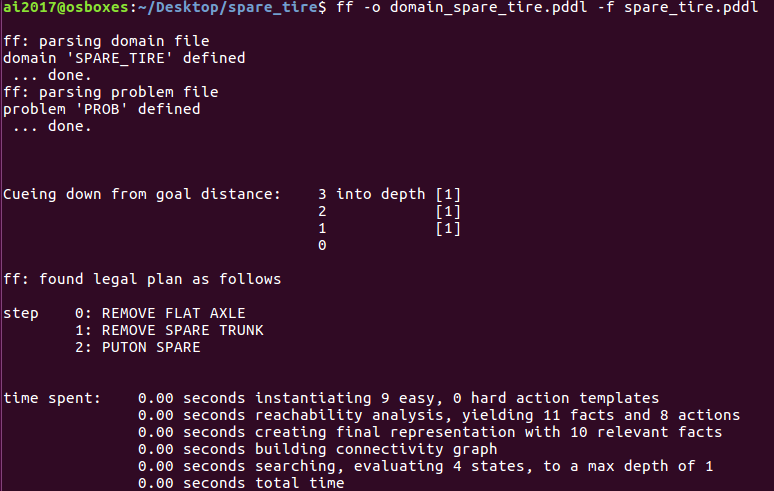
\includegraphics[width=16cm]{Pic/spare_tire}
\end{figure}

\subsection{Briefcase World}
\label{sec:briefcase-world}

Please refer to \texttt{pddl.pdf} at page 2. Please pay More attention to the usages of \texttt{forall} and \texttt{when}.  

For more examples, please refer to \texttt{ff-domains.tgz} and \texttt{benchmarksV1.1.zip}. For more usages of FF planner, please refer to the documentation \texttt{pddl.pdf}.
\section{Tasks}

\subsection{8-puzzle}
\begin{figure}[ht]
  \centering
  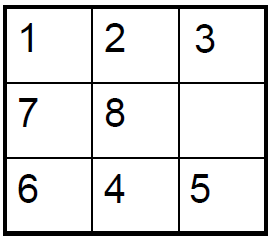
\includegraphics[width=0.4\textwidth]{Pic/puzzle}
  \qquad
  \parbox[b]{0.4\textwidth}{Please complete  \texttt{domain\_puzzle.pddl} and \texttt{puzzle.pddl} to solve the 8-puzzle problem.\\}
\end{figure}
\label{sec:8-puzzle}
\begin{lstlisting}[title=domain\_puzzle.pddl,frame=single,language=lisp,numbers=left]
(define (domain puzzle)
  (:requirements :strips :equality:typing)
  (:types num loc) 
  (:predicates  ())

(:action slide
             :parameters ()
             :precondition ()
             :effect () 
 )
)
\end{lstlisting}
\begin{lstlisting}[title=domain\_puzzle.pddl,frame=single,language=lisp,numbers=left]
(define (problem prob)
 (:domain puzzle)
 (:objects )
 (:init )
 (:goal ())
)

\end{lstlisting}
\subsection{Blocks World}
Planning in the blocks world is a traditional planning exercise, and you can recall what we have introduced in the theory course.
\\ There are a collection of blocks: a block can be on the table, or on the top of another block. 
\\ There are three predicates:  
\begin{itemize}

\item\textit{clear(x)}: there is no block on top of block x;

\item \textit {on(x,y)}: block x is on the top of block y;

\item   \textit {onTable(x)}: block x is on the table

\end{itemize}There are two actions in this task:
\begin{itemize}

\item\textit{move(x,y)}: move block x onto block y, provided that both x and y are clear;

\item \textit {moveToTable(x)}: move block x on to the table, provided that x is clear and x is not on the table;

\end{itemize}Give initial state and goal state, find the actions change the initial state to the goal state.
\\
\\
In this task, please complete the file \texttt{domain\_blocks.pddl} to solve the blocks world problem. You should know the usages of \texttt{forall} and \texttt{when}.

\begin{lstlisting}[title=domain\_blocks.pddl,frame=single,language=lisp,numbers=left]
(define (domain blocks)
  (:requirements :strips :typing:equality
                 :universal-preconditions
                 :conditional-effects)
  (:types physob)
  (:predicates   
  	    (ontable ?x - physob)
            (clear ?x - physob)	
	    (on ?x ?y - physob))
		
  (:action move
             :parameters (?x ?y - physob)
             :precondition ()
             :effect ()
             )

  (:action moveToTable
             :parameters (?x - physob)
             :precondition ()
             :effect ( )
 )



\end{lstlisting}

\label{sec:problem-description}

\begin{lstlisting}[title=blocks.pddl,frame=single,language=lisp,numbers=left]
(define (problem prob)
 (:domain blocks)
 (:objects A B C D E F - physob)
 (:init (clear A)(on A B)(on B C)(ontable C) (ontable D)
  (ontable F)(on E D)(clear E)(clear F)
)
 (:goal  (and (clear F) (on F A) (on A C) (ontable C)(clear E) (on E B) 
         (on B D) (ontable D)) )
 )




\end{lstlisting}
Please submit a file named \textsf{E06\_YourNumber.pdf}, and send it to \textsf{ai\_2020@foxmail.com}


\section{Codes and Results}

\subsection{8-puzzle}


\begin{lstlisting}[title=domain\_puzzle.pddl,frame=single,language=lisp,numbers=left]
(define (domain puzzle)
    (:requirements
        :strips :equality :typing)
    (:predicates
        (tile ?x) (position ?x)
        (at ?t ?x ?y) (blank ?x ?y)
        (add ?new ?pre) (sub ?new ?pre))
        
     (:action up
     :parameters (?t ?x ?y ?x_new)
     :precondition (
         and (tile ?t) (position ?x) (position ?y) (position ?x_new)
        	    (sub ?x_new ?x) (blank ?x_new ?y) (at ?t ?x ?y))
     :effect (
         and (not (blank ?x_new ?y)) (not (at ?t ?x ?y))
        	    (blank ?x ?y) (at ?t ?x_new ?y)))
        	     
    (:action down
    :parameters (?t ?x ?y ?x_new)
    :precondition (
        and (tile ?t) (position ?x) (position ?y) (position ?x_new)
        	   (add ?x_new ?x) (blank ?x_new ?y) (at ?t ?x ?y))
    :effect (and (not (blank ?x_new ?y)) (not (at ?t ?x ?y))
        	   (blank ?x ?y) (at ?t ?x_new ?y)))
        	   
    (:action left
    :parameters (?t ?x ?y ?y_new)
    :precondition (
        and (tile ?t) (position ?x) (position ?y) (position ?y_new)
    	       (sub ?y_new ?y) (blank ?x ?y_new) (at ?t ?x ?y))
    :effect (
        and (not (blank ?x ?y_new)) (not (at ?t ?x ?y))
               (blank ?x ?y) (at ?t ?x ?y_new)))
               
    (:action right
    :parameters (?t ?x ?y ?y_new)
    :precondition (
        and (tile ?t) (position ?x) (position ?y) (position ?y_new)
    	       (add ?y_new ?y) (blank ?x ?y_new) (at ?t ?x ?y))
    :effect (
        and (not (blank ?x ?y_new)) (not (at ?t ?x ?y))
               (blank ?x ?y) (at ?t ?x ?y_new)))
)

\end{lstlisting}
\begin{lstlisting}[title=domain\_puzzle.pddl,frame=single,language=lisp,numbers=left]
(define (problem prob)
    (:domain puzzle)
    (:objects t1 t2 t3 t4 t5 t6 t7 t8 p1 p2 p3 q1 q2 q3)
    (:init (tile t1) (tile t2) (tile t3) (tile t4)
           (tile t5) (tile t6) (tile t7) (tile t8)
           (position p1) (position p2) 
           (position p3) (position q1) 
           (position q2) (position q3)
           (blank p2 q3)
           (at t1 p1 q1) (at t2 p1 q2) (at t3 p1 q3) (at t7 p2 q1)
           (at t8 p2 q2) (at t6 p3 q1) (at t4 p3 q2) (at t5 p3 q3)
           (add p2 p1) (add p3 p2) (sub p1 p2) (sub p2 p3)
           (add q2 q1) (add q3 q2) (sub q1 q2) (sub q2 q3) )
    (:goal (
        and (at t1 p1 q1) (at t2 p1 q2) (at t3 p1 q3) (at t4 p2 q1)
            (at t5 p2 q2) (at t6 p2 q3) (at t7 p3 q1) (at t8 p3 q2)
            (blank p3 q3) ))
)
\end{lstlisting}

Results:

\begin{figure}[ht]
  \centering
  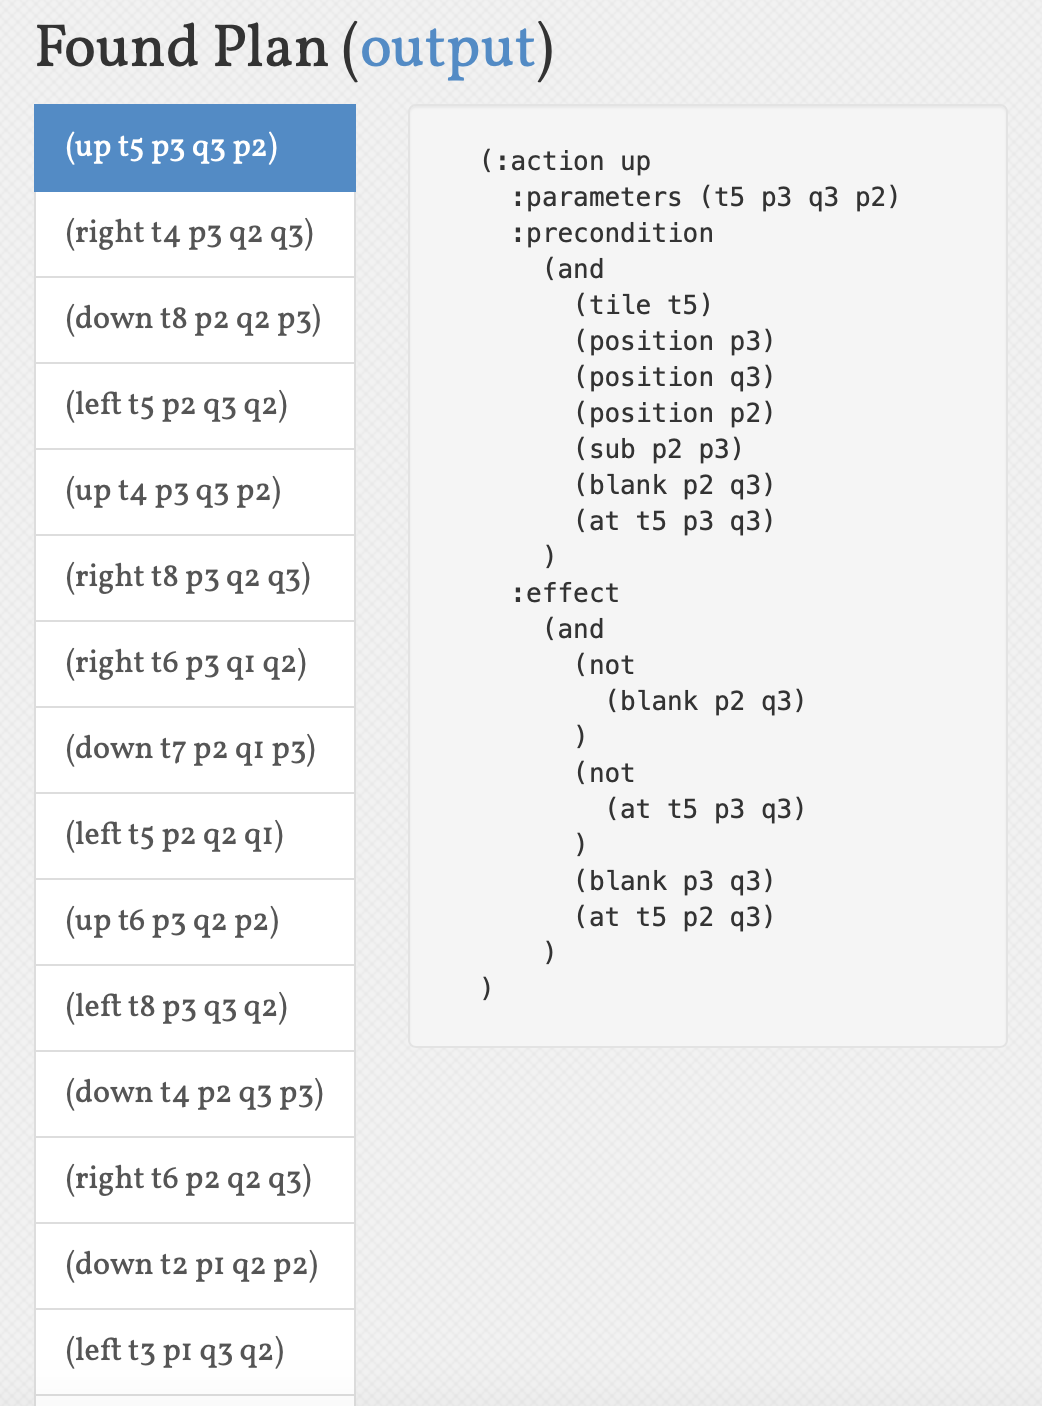
\includegraphics[width=0.6\textwidth]{Pic/1}
  \qquad
  \parbox[b]{0.6\textwidth}{Part of the result on the website\\}
\end{figure}
All results:
\begin{lstlisting}[title=result1,frame=single,numbers=left]
(up t5 p3 q3 p2)
(right t4 p3 q2 q3)
(down t8 p2 q2 p3)
(left t5 p2 q3 q2)
(up t4 p3 q3 p2)
(right t8 p3 q2 q3)
(right t6 p3 q1 q2)
(down t7 p2 q1 p3)
(left t5 p2 q2 q1)
(up t6 p3 q2 p2)
(left t8 p3 q3 q2)
(down t4 p2 q3 p3)
(right t6 p2 q2 q3)
(down t2 p1 q2 p2)
(left t3 p1 q3 q2)
(up t6 p2 q3 p1)
(up t4 p3 q3 p2)
(right t8 p3 q2 q3)
(down t2 p2 q2 p3)
(left t4 p2 q3 q2)
(down t6 p1 q3 p2)
(right t3 p1 q2 q3)
(up t4 p2 q2 p1)
(right t5 p2 q1 q2)
(down t1 p1 q1 p2)
(left t4 p1 q2 q1)
(up t5 p2 q2 p1)
(up t2 p3 q2 p2)
(right t7 p3 q1 q2)
(down t1 p2 q1 p3)
(down t4 p1 q1 p2)
(left t5 p1 q2 q1)
(up t2 p2 q2 p1)
(right t4 p2 q1 q2)
(up t1 p3 q1 p2)
(left t7 p3 q2 q1)
(down t4 p2 q2 p3)
(right t1 p2 q1 q2)
(down t5 p1 q1 p2)
(left t2 p1 q2 q1)
(up t1 p2 q2 p1)
(right t5 p2 q1 q2)
(down t2 p1 q1 p2)
(left t1 p1 q2 q1)
(up t5 p2 q2 p1)
(right t2 p2 q1 q2)
(up t7 p3 q1 p2)
(left t4 p3 q2 q1)
(down t2 p2 q2 p3)
(right t7 p2 q1 q2)
(up t4 p3 q1 p2)
(left t2 p3 q2 q1)
(down t7 p2 q2 p3)
(down t5 p1 q2 p2)
(right t1 p1 q1 q2)
(up t4 p2 q1 p1)
(up t2 p3 q1 p2)
(left t7 p3 q2 q1)
(down t5 p2 q2 p3)
(right t2 p2 q1 q2)
(down t4 p1 q1 p2)
(left t1 p1 q2 q1)
(up t2 p2 q2 p1)
(up t5 p3 q2 p2)
(left t8 p3 q3 q2)
\end{lstlisting}

\subsection{Blocks World}

\begin{lstlisting}[title=domain\_blocks.pddl,frame=single,language=lisp,numbers=left]
(define (domain blocks)
    (:requirements
        :strips :equality :typing
        :universal-preconditions
        :conditional-effects)
    (:types physob)
    (:predicates 
        (ontable ?x - physob)
        (clear ?x - physob)
        (on ?x ?y - physob))
        
    (:action move
        :parameters (?x ?y - physob)
        :precondition(
            and (clear ?x) (clear ?y) (not (= ?x ?y)))
        :effect(
            and (forall (?z - physob)
                    (when (on ?x ?z) (
                        and (not (on ?x ?z)) (clear ?z) ))) 
                (not (clear ?y)) (on ?x ?y) (not (ontable ?x))))
                
    (:action moveToTable
        :parameters (?x - physob)
        :precondition(
            and (clear ?x) (not (ontable ?x)))
        :effect( and (ontable ?x) ))
)




\end{lstlisting}

\label{sec:problem-description}

\begin{lstlisting}[title=blocks.pddl,frame=single,language=lisp,numbers=left]
(define (problem prob)
 (:domain blocks)
 (:objects A B C D E F - physob)
 (:init (clear A)(on A B)(on B C)(ontable C) (ontable D)
  (ontable F)(on E D)(clear E)(clear F)
)
 (:goal  (and (clear F) (on F A) (on A C) (ontable C)(clear E) (on E B) 
         (on B D) (ontable D)) )
 )

\end{lstlisting}
Results:
\begin{figure}[ht]
  \centering
  
\includegraphics[width=0.6\textwidth]{Pic/2}
  \qquad

\end{figure}

%\clearpage
%\bibliography{E:/Papers/LiuLab}
%\bibliographystyle{apalike}
\end{document} 
%%% Local Variables:
%%% mode: latex
%%% TeX-master: t
%%% End:
